
\section{Droplet Horizontal View}

\par The main objective of this experiment was to observe qualitatively the heat gradients in the droplet as it collides with the heated surface and removes its heat. To create a heater, cartridge resistance heaters were put under an aluminum plate, radiating to its surface. The experiment was made for water droplets, and the surface was hydrophilic. \\

\par To minimize the surface roughness interference a silica wafer was used, thus assuring a droplet fall as symmetric as possible. In the interface of the silica wafer and the aluminum plate a thermal paste was used to improve heat transfer. On top of the silica wafer there is a thermocouple that tracks the surface temperature. This setup can be seen in detail in Figure \ref{fig:horizontal2}. The thermocouple value is used by a PID controller to control the heat released by the cartridge heater. In the PID's screen the temperature of the plate is at its top and the target temperature at the bottom.\\

\begin{figure}[h]
\centering
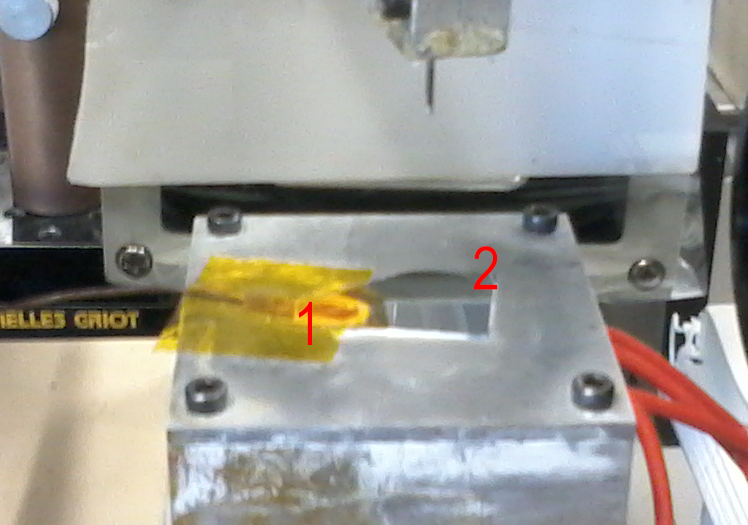
\includegraphics[width=0.5\linewidth]{Figures/3.Chapter/horizontal2.png}
\caption{Silica wafer setup: (1) Thermocouple, (2) Silica Wafer}
\label{fig:horizontal2}
\end{figure}

\par An Harvard Apparatus controls a syringe's water discharge, that then falls from the needle to the wafer. This forms a droplet with 2.6 to 3 mm diameter spherical droplet. This experiment is recorded by 2 cameras: IR camera and high-speed camera. In order for the high-speed camera to work, a high intensity lamp is also needed. The described setting can be seen in Figure \ref{fig:horizontal}. This setting was used to gather qualitative results only. Good quantitative results are impossible due to the implications of droplet geometry in thermography.

\begin{figure}[h]
\centering
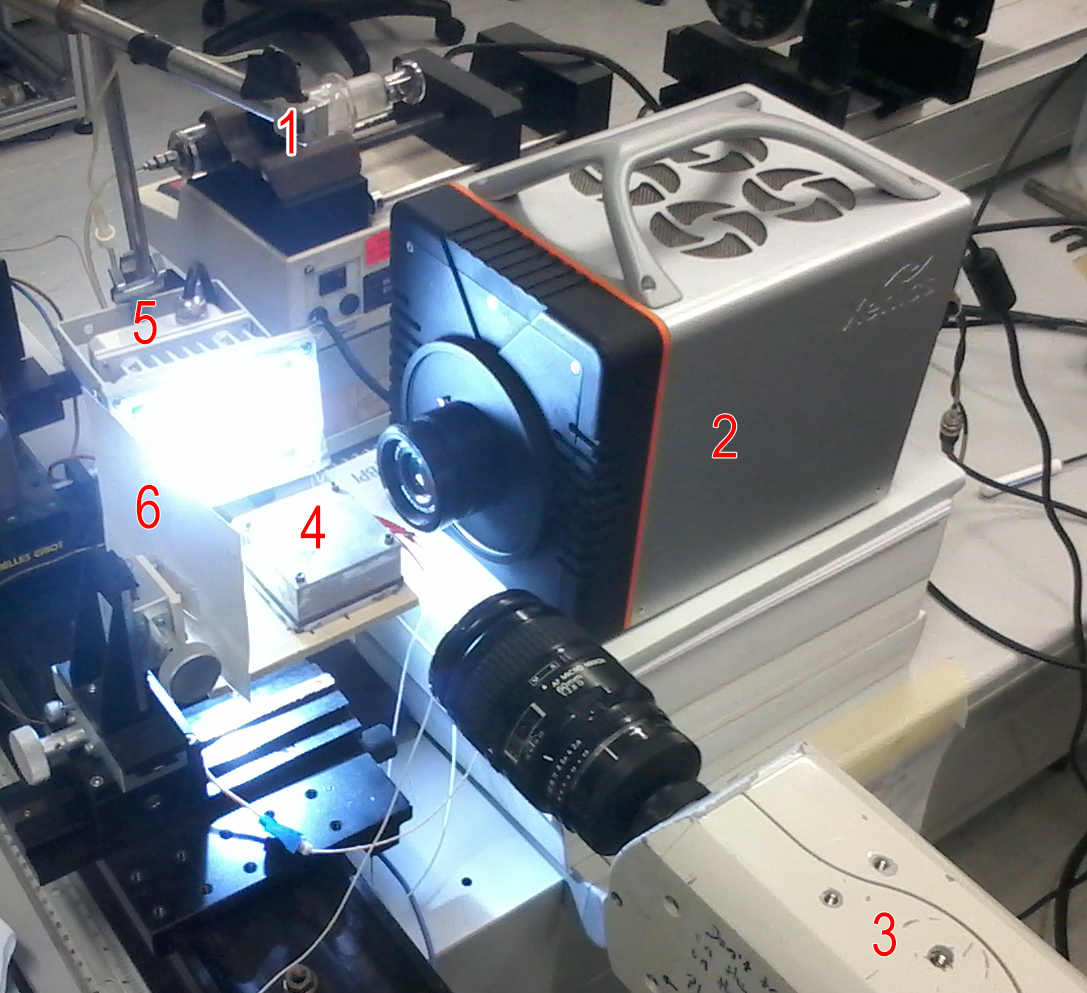
\includegraphics[width=0.65\linewidth]{Figures/3.Chapter/horizontal.png}
\caption{Horizontal setup: (1) Needle, (2) IR Camera, (3) HS Camera, (4) Heated Surface, (5) Lamp, (6) Black Background}
\label{fig:horizontal}
\end{figure}

\subsection{Procedure}
\label{sec:procedure}
\begin{itemize}
\item Adjust IR Camera's settings on the software.
\item Perform an offset calibration (described in Section \ref{sec:icam}).
\item Adjust PID controller to the desired temperature and water flow in the Harvard Apparatus.
\item Turn on the light and set the cameras recording.
\item Let a droplet drop on the wafer.
\item Clean the wafer with acetone and distilled water before proceeding.
\end{itemize}

\section{Droplet Bottom View}

\par The objective of this setup is to observe interface temperatures in during the droplet impact phases. To do this, the IR Camera had to be placed underneath the surface in which the droplet impacts. The droplet impacts on a 20 $\mu m$ thick stainless steel foil. This was done similarly to \cite{sielaff2014experimental}, as the objective was to read the interface temperatures. Because of the small thickness of the foil, the temperature of the interface is very similar to the read temperature in the bottom of the foil. The HS camera was placed horizontally to the foil to observe the impact. A lamp was placed in the opposite site. The setup scheme can be seen in Figure \ref{fig:setup}.\\

\begin{figure}[h]
\centering
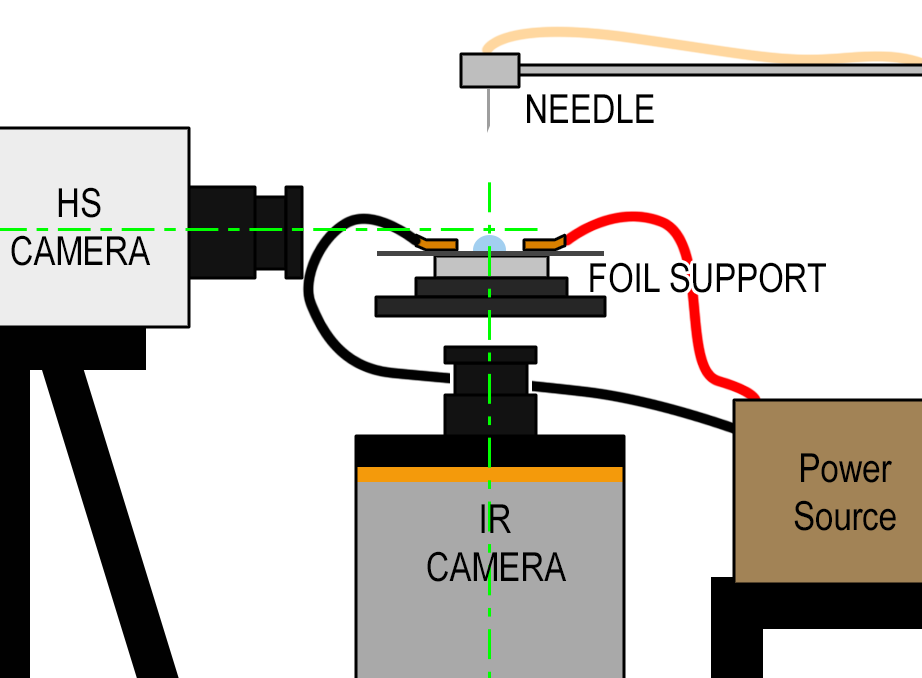
\includegraphics[width=0.55\linewidth]{Figures/3.Chapter/setup.png}
\caption{Bottom Setup Scheme}
\label{fig:setup}
\end{figure}

\par The experiments made around this setup were made using hydrophilic (using distilled water and ethanol) and super-hydrophobic (using just water) surfaces. A preliminary experiment with water and an hydrophilic surface was made, using the software calibration. From the first, raw results were taken for posterior calibration and processing. The calibrations and their differences are explained in Chapter \ref{cap:setup}.\\

\par The foil is fed an electric current, so it can heat up to the desired temperature. This is done by to electrical contacts, wired to a power source. The foil has to be placed on top of a bad heat conductor to minimize heat losses. A heat glass was chosen for the purpose. It also needs to be stretched so that possible wrinkles don't affect the droplet. A detail of the setup, on the foil support can be seen in Figure \ref{fig:suporte}. In this figure two supports are shown. The second was made after the calibration. \\

\par For the case of the super-hydrophobic surfaces, the surfaces needed to be cleaned with an ultra-sound bath and coated with \textit{Glaco}. This coating took several layers to ensure effective coating that can endure high temperature and constant droplet fall. \\

\begin{figure}[h]
\centering
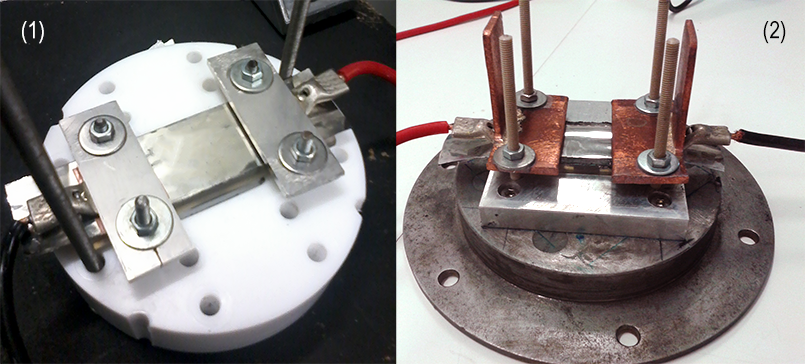
\includegraphics[width=0.9\linewidth]{Figures/3.Chapter/suporte.png}
\caption{Stainless Steel Support: (1) Before calibration setup, (2) After calibration setup}
\label{fig:suporte}
\end{figure}

\par This setup also has the Harvard Apparatus and the needle to create the droplet. A metal structure holds the support, needle and camera. The complete setup can be seen in Figure \ref{fig:setup2}. Although we have a different calibration, the procedure is similar to the previously described in \ref{sec:procedure}. The big difference is that the foil temperature is controlled with the power source and not with the PID. To adjust the current correctly one needs to read the temperature on the IR Camera's software. In the case that raw images are needed, an additional step should be to convert the desired temperatures in ADU. Only this way one can know if the foil is at the desired temperature.

\begin{figure}[h]
\centering
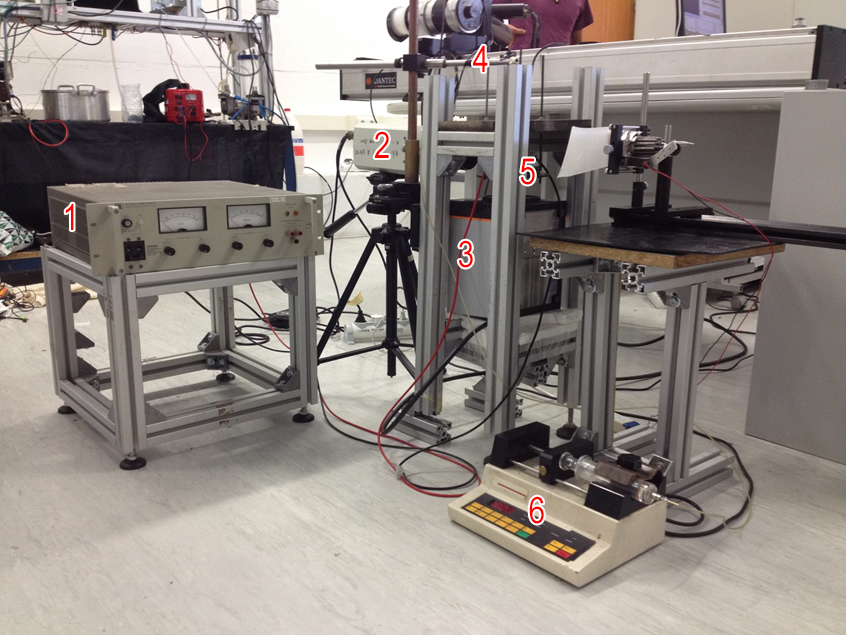
\includegraphics[width=0.9\linewidth]{Figures/3.Chapter/setup2.png}
\caption{Bottom Setup: (1) Power Source, (2) HS Camera, (3) IR Camera, (4) Needle, (5) Foil Support, (6) Harvard Apparatus}
\label{fig:setup2}
\end{figure}